\subsubsection{Positively correct the plasmidness}\label{sec:pbf_iterbin:decomp:mps:fine_tuned}

Especially when \(\omega_c\) is inferior than the sum, if the flow passes through the fragment path corresponding to this contig, we would like to positively correct the sum to obtain \(\omega_c\).

In what follows, we associate new attributes to the fragments corresponding to the possible positive correction we may add to the objective values.
We then adapt the MILP formulations for the corrections.

\begin{refactorbox}
  The idea of correction/bonus is shared between the GC penalties and the plasmidness.
  Restructure to show the common parts and argue in favour of the bonuses.
\end{refactorbox}

\begin{fixmebox}
  Argument order for plasmidness bonus
\end{fixmebox}

Let \(c_1\) and \(c_2\) be two contigs that share a fragment \(j\), where \(\frac{ |j| }{ |c_1| } \rho_{c_1} \geq \frac{ |j| }{ |c_2| } \rho_{c_2}\)
For simplicity, suppose their fragment sets only contain one share, which is \(j\), and \(j\) does not belong to any other contig (i.e. \(\Contigs(j) = \{c_1, c_2\} \)).
Then:
\[
  \sum_{i \in \Fragments{}(c_1) } \rho_{i} = \plm{j} + \sum_{i \in \Fragments{}(c_1), i \neq j} \frac{ |i| }{ |c_1| } \rho_{c_1} \leq \rho_{c_1} = \sum_{i \in \Fragments{}(c_1) } \frac{ |i| }{ |c_1| } \rho_{c_1}
\]

The difference between the two inequality parts equals to:
\[
  \rho_{c_1} - \sum_{i \in \Fragments{}(c_1) } \rho_{i} = \frac{ |j| }{2} \left(\frac{ \rho_{c_1} }{ |c_1| } - \frac{ \rho_{c_2} }{ |c_2| } \right) \geq 0
\]

If the flow passes through all the link-arcs that define \(c_1\) (links in \(A_\Links{}(c_1)\) or links in \(A_\Links{}(\rev{c_1})\) for the reverse of \(c_1\)), the plasmidness is penalized because of the fragmentation of \(c_1\), particularly because of the plasmidness of the share \(j\).
Without the fragmentation of the contig \(c_1\), the plasmidness would have been higher by the difference.

In the following we present a way to solve this issue.

For all share \(j \in \Fragments{}\), we can define a correction constant relative to a contig \(c \in \Contigs(j)\):
\[
  \dplm{c}{j} = \max \Set*{0, \frac{ |i| }{ |c| }\plm{c} - \plm{j}}
\]

If the flow passes through all the link-arcs defining \(c\) (or its reverse), we positively correct the objective value by \(\dplm{c}{j}\).
When the flow passes through several contigs in \(\Contigs(j)\), we only add once this bonus to the objective value, and this bonus is the best of the \(\dplm{c}{j}\) among the \(c \in \Contigs(j)\), represented by the variable \(\rho cor_j\).

\zcref[S]{fig:correct_share_plasmidness} illustrates the values of the share plasmidness correction variables.

\begin{figure}[htb]
  \centering
  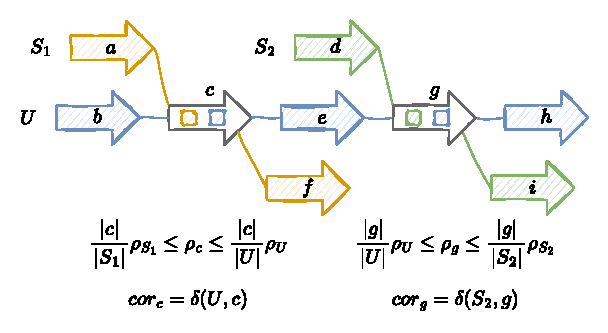
\includegraphics[width=0.6\linewidth]{appendix/ideas/asmcons_milp_fine_tuning/img/constraints-correct_plasmidness_example.pdf}
  \figurecaption{Differential correction of share fragment plasmidness.}{%
    Let assume the flow passes through all the link-arcs defining contigs \(U\), \(S_1\) and \(S_2\) (or their reverse).
    Because of the inequalities between the plasmidness, the objective function is corrected by \(\dplm{U}{c}\) for the share \(c\), and by \(\dplm{S_2}{g}\) for the share \(g\).
  }\label{fig:correct_share_plasmidness}
\end{figure}

\begin{todobox}
  Adapt best bonus GC prob score for plasmidness
\end{todobox}